% !TEX root = ../main.tex
\begin{figure}[h]
\centering
\iflatexml
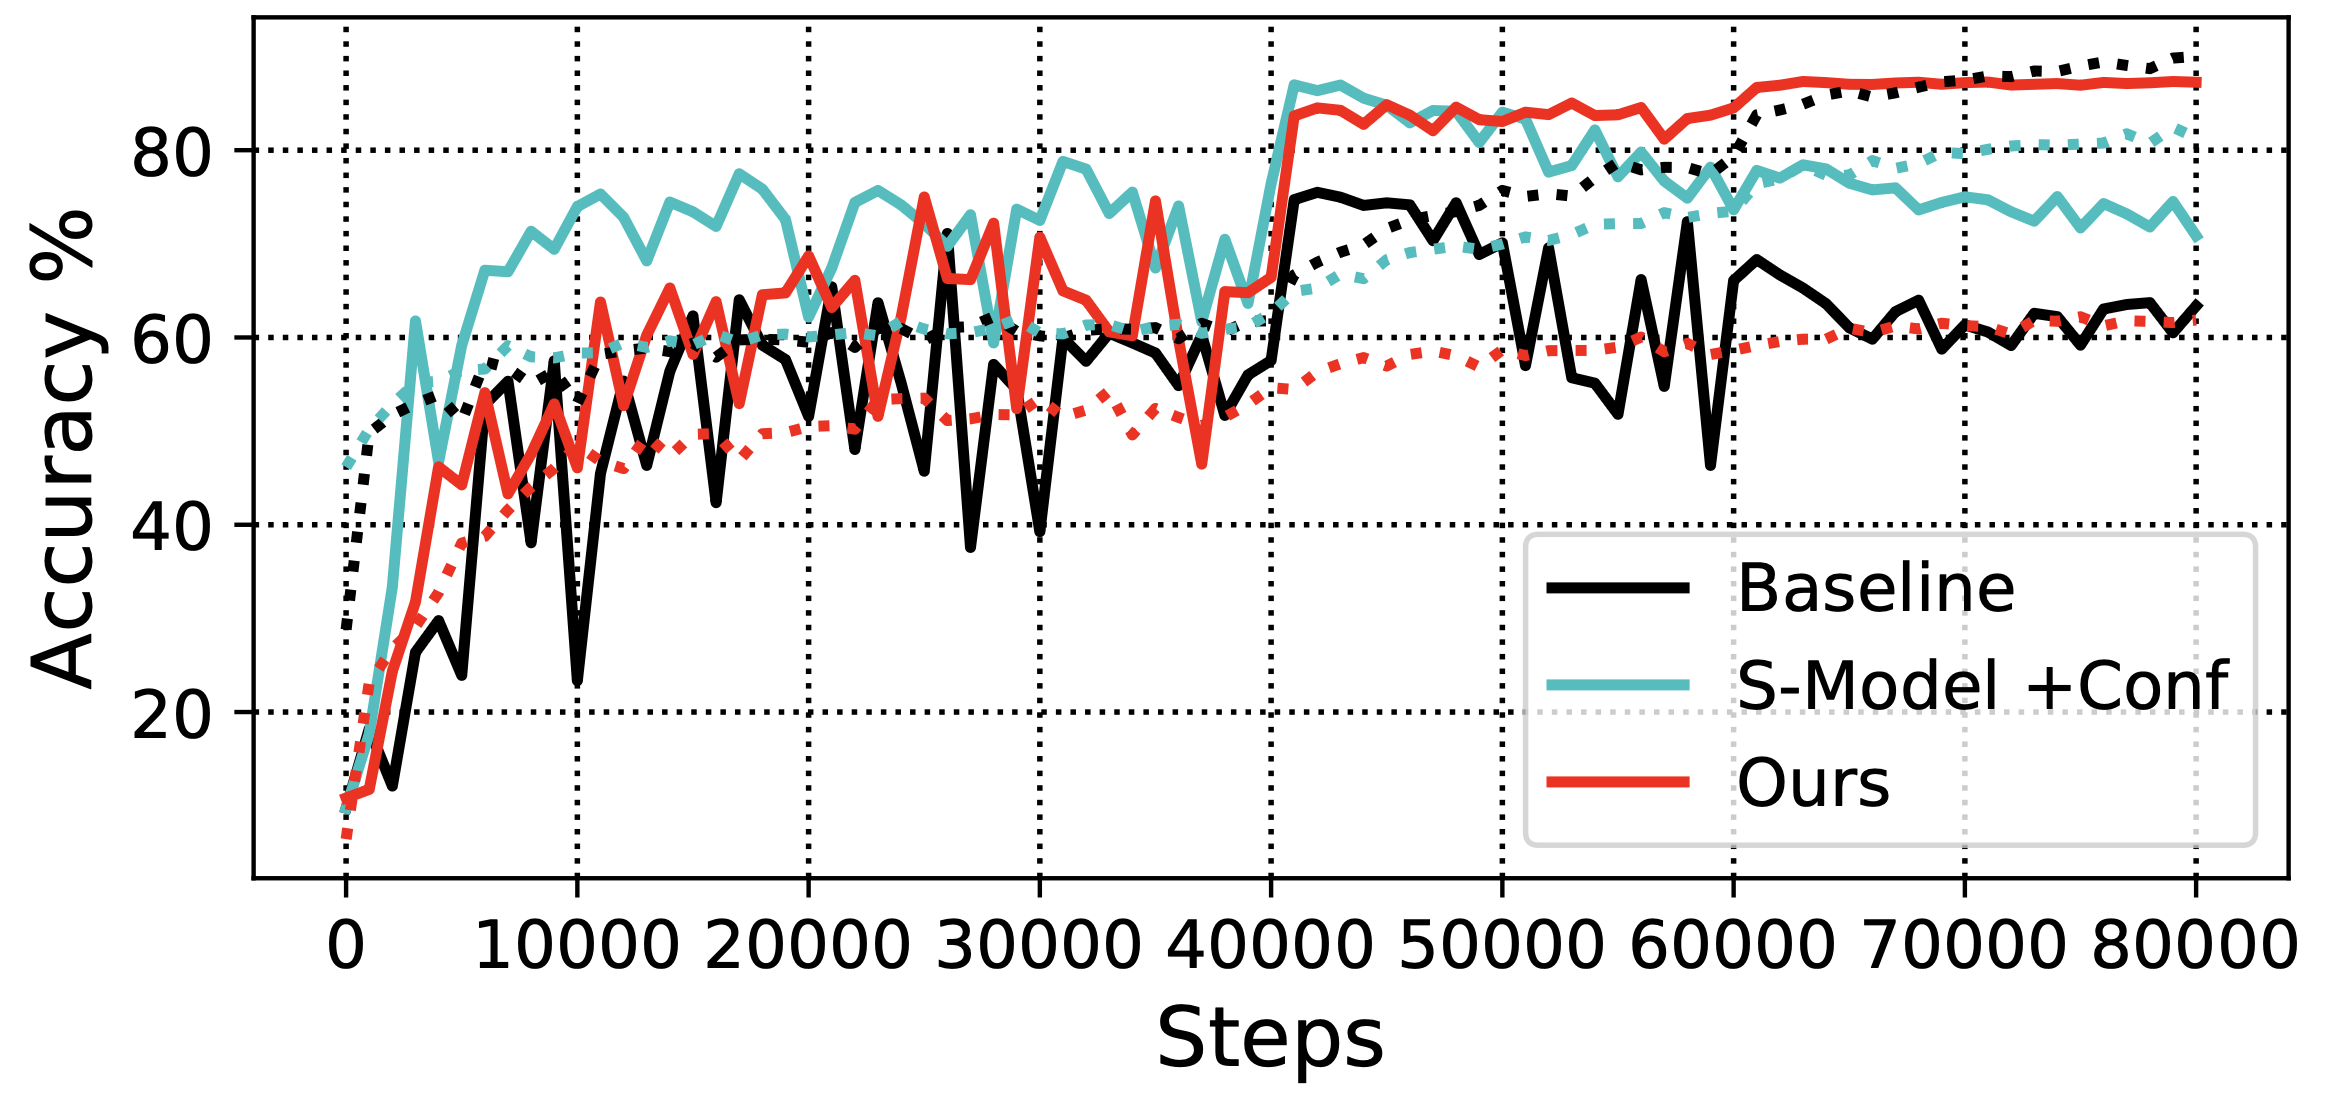
\includegraphics[width=6\columnwidth]{figures/cifar-10-curve.png}
\else
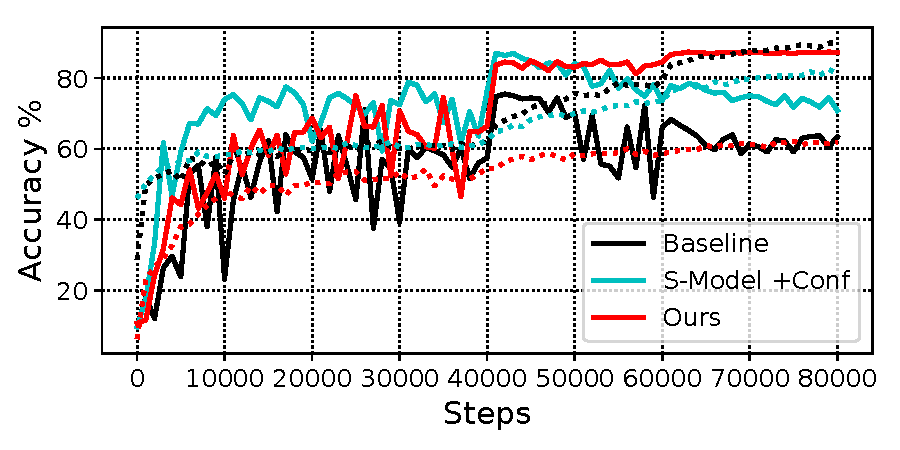
\includegraphics[width=0.9\columnwidth]{figures/cifar-10-curve.pdf}
\fi
\vspace{-0.1in}
\caption{Training curve of a ResNet-32 on CIFAR-10 \textsc{BackgroundFlip} under 40\% noise ratio.
Solid lines denote validation accuracy and dotted lines denote training. Our method is less prone to
label noise overfitting.}
\label{fig:curve}
\vspace{-0.15in}
\end{figure}
